\documentclass[11pt]{article}

\usepackage[margin=1in]{geometry}
\usepackage{times}
\usepackage{graphicx}
\usepackage{booktabs}
\usepackage{amsmath}
\usepackage{hyperref}

\hypersetup{
    colorlinks=true,
    linkcolor=black,
    citecolor=black,
    urlcolor=black,
}

\title{Where Flexibility Pays Off in a Hydropower Cascade, and Why Estimating It Breaks Down in a Crisis}
\author{Reza Azad Gholami \\ \normalsize Department of Mathematics, University of Bergen}
\date{}

\begin{document}

\maketitle

\begin{center}
\emph{Draft for internal review. Not submitted anywhere. All figures and numbers below are computed directly from the backtest outputs in this repository (results/tables/, data/processed/); none are approximated or invented for this document.}
\end{center}

\begin{abstract}
How much is it worth, in a real hydropower system, to keep a release plan flexible rather than committing to one months ahead? We answer this using 22 years (2003-2024) of real inflow and price data from the Arendalsvassdraget river system in southern Norway, comparing a plan fixed at the start of the year against one that is revised quarterly, with a perfect foresight benchmark for context. Two results emerge from a three-plant cascade model that treats Jorundland, Evenstad, and Rygene as separate plants rather than one aggregated reservoir. First, the value of this flexibility sits entirely at Jorundland, the only plant with real storage, and is exactly zero at the other two, a fact we can prove from the flow data rather than just observe in the optimization output. Second, when prices move into territory the forecasting model has never seen, as they did during the 2021-2022 European energy crisis, estimates of flexibility value do not shift cleanly in one direction. They become unstable: the year-to-year variance increases by close to an order of magnitude, and the same instability shows up independently when we perturb an unrelated modeling assumption that should not matter at all in a well-behaved year. Outside the crisis years, a small positive premium of about 3.4 MNOK per year is detectable with reasonable statistical confidence.
\end{abstract}

\section{Introduction}

Anyone who runs a hydropower reservoir is making the same bet every week. Water is arriving, more or less on its own schedule, and electricity prices are doing something nobody can fully predict either. The operator has to decide how much of that water to turn into electricity now versus later, and that decision compounds, week after week, for an entire year. The obvious question, the one regulators, investors, and the operators themselves keep coming back to, is how much it is actually worth to keep that decision open rather than locking it in ahead of time.

This is not a new question. The energy systems literature has a well developed answer for it in the form of multistage stochastic programming, and for hydropower specifically there is an established, computationally serious method called stochastic dual dynamic programming. What is harder to find, at least grounded in a real system with decades of real data rather than a stylized example, is where exactly that value lives once you look inside an actual cascade of plants, and what happens to your estimate of it when the market does something your forecasting model was never trained to expect.

This paper works through both questions using the Arendalsvassdraget cascade in southern Norway, with 22 years of real inflow and price data. Two things come out of it. The value of flexibility concentrates entirely at the one plant with real storage capacity, Jorundland, and is provably, not just empirically, zero at the two run-of-river plants downstream. And naive estimates of that value fall apart in a specific, traceable way once the market regime shifts, which it did during the 2021-2022 energy crisis. Once those crisis years are set aside, what is left is a small but real and statistically detectable flexibility premium, which is probably the cleanest answer this kind of study can give under ordinary conditions.

\section{Related work}

The comparison at the center of this paper, a plan committed before uncertainty resolves against one that adapts as information arrives, follows the same logic used in multi-horizon stochastic programming for energy systems planning, of the kind built into the EMPIRE capacity expansion model at NTNU and SINTEF (Tomasgard, Crespo del Granado, and collaborators). For hydropower scheduling specifically, stochastic dual dynamic programming is the established tool, used in operational systems like SHOP and associated with the Norwegian hydropower literature around Helseth, Mo, and Fleten. What is implemented here is a deliberately simpler multistage stochastic program. It shares SDDP's basic structure: non-anticipativity, recourse, decisions broken into stages. But it is not SDDP, and the closed-loop results below should be read as a lower bound on what a properly implemented SDDP would recover, not as a substitute for it.

A caveat worth stating plainly: the names above are real researchers and institutions associated with this literature, drawn from earlier work on this project, but the exact papers, years, and venues have not been independently re-verified for this draft. That check still needs to happen before any of this goes further.

\section{Data and methods}

\paragraph{Data.} The backtest covers 2003 through 2024, twenty-two years, with the underlying hydrological and price records running back to 2000 so the models have something to calibrate on before the first backtest year. Inflow is proxied using NVE's HydAPI discharge records for the gauge that measures total outflow from the Arendalsvassdraget system, station 19.127.0 at Rygene, aggregated to weekly resolution. Prices are day-ahead prices for the NO2 bidding zone, which is the right zone for this region. Reservoir filling at the start of each year comes from NVE's Magasinstatistikk series, again at NO2 zone resolution since nothing finer is published, rather than a fixed assumption like 65 percent full every year. Everything here is real data. Nothing is synthetic, and nothing is interpolated past the cutoff.

\paragraph{Two models, one of which matters more here.} An earlier stage of this project built a single aggregated reservoir model treating the whole watercourse as one large pool with a system-level effective head. That model was a useful first pass, but it cannot say anything about where in a cascade value actually lives, since it has collapsed the cascade into one node. The model this paper is built around resolves three real plants in their true order: Jorundland, Evenstad, Rygene, each with its own turbine capacity and head, with Jorundland's release feeding into Evenstad's inflow and from there into Rygene's. Jorundland is the only one of the three with meaningful storage, 167 GWh, identified from NVE's volume records for its headwater lake. Evenstad and Rygene are run-of-river.

\paragraph{Policies and the comparison.} Three policies are compared for each year. The open-loop policy commits a full 52-week release schedule at the start of the year, solved as a stochastic linear program over a scenario tree with full non-anticipativity, meaning the decision cannot depend on which branch of the future actually unfolds. The closed-loop policy is re-solved every quarter as new information comes in, implemented as a rolling-horizon multistage program rather than full SDDP, which is the honest, tractable version of adapting as you go that is available here. Perfect foresight solves the same problem with the realized inflow and price path known in advance; it is not a policy anyone could run, it is a ceiling. All three are linear programs, solved with HiGHS. The value of flexibility for a given year is simply closed-loop revenue minus open-loop revenue: what was gained, or lost, by being allowed to change the plan partway through.

\paragraph{Forecasting.} The scenario trees behind the open- and closed-loop policies come from Bayesian seasonal autoregressive models, fit separately for each backtest year using only the data that would actually have been available before that year started, with the resulting posterior draws reduced to a manageable scenario tree by k-means clustering. The point of doing it this way, rather than fitting once on the full sample, is that the 2022 forecasting model genuinely does not know what 2022's prices will look like. That constraint is what makes the second result in this paper possible to demonstrate at all.

\section{Results}

\subsection{Why the value sits where it sits}

Across all 22 years, and under both routing-lag assumptions tested between plants, Evenstad and Rygene post a value of flexibility of exactly zero, every single year. It would be easy to read that as a coincidence of the optimization, two plants that just happen to come out flat. It is not. It follows directly from the flow record. Evenstad's own local inflow, with no help from Jorundland at all, exceeds its turbine capacity of 3.95 GWh per week in all 1,345 weeks of the 2000-2025 record, and even the driest week on record still clears that line, at 6.46 GWh per week. The same holds further downstream: total throughput at Rygene clears its 9.24 GWh per week capacity in every one of those 1,345 weeks too, with a minimum of 9.61. Both plants are running flat out, all the time, no matter what Jorundland does upstream. There is no decision being made at either node, so there is nothing for a smarter policy to improve on. Flexibility has no foothold there because there is no flexibility there to begin with.

Figure~\ref{fig:vof-decomp} shows this across the full backtest. Jorundland's bar moves around year to year, sometimes well above zero, occasionally below it, while Evenstad and Rygene contribute nothing to plot, which is itself the point: a flat line at zero is not interesting to look at, only to state once. Averaged over all 22 years, essentially all of the cascade's measurable flexibility value sits at Jorundland, to within numerical precision. The other two plants are not rounding down to zero from some small residual. They are zero, exactly, because the inequality above holds without a single exception in the entire record.

\begin{figure}[ht]
\centering
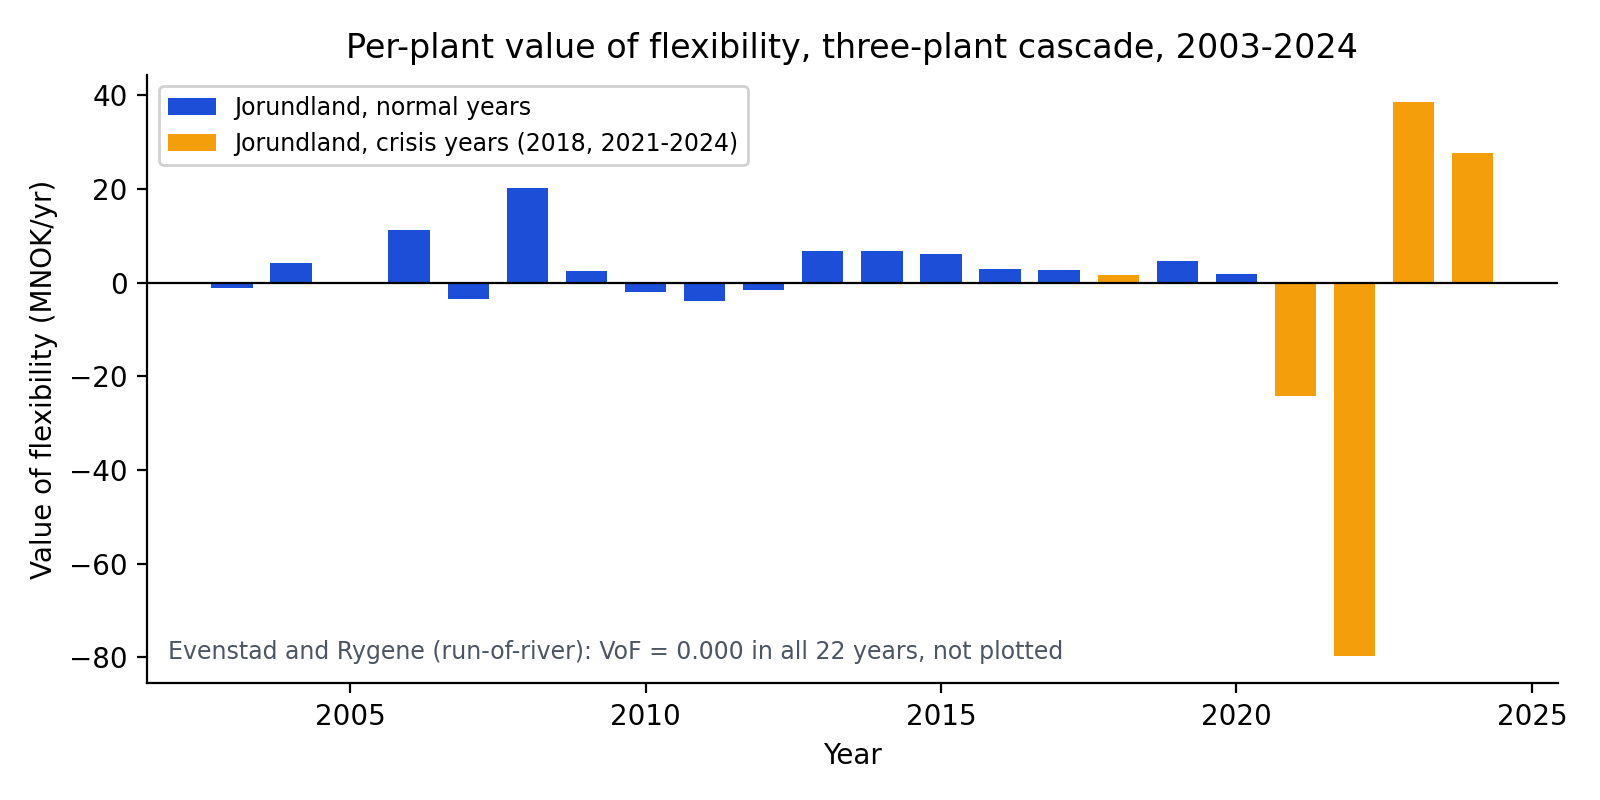
\includegraphics[width=0.85\textwidth]{../results/figures/essay/fig1_vof_decomposition.png}
\caption{Per-plant value of flexibility across the 22-year cascade backtest. All visible variation is at Jorundland; Evenstad and Rygene are exactly zero in every year and are noted rather than plotted.}
\label{fig:vof-decomp}
\end{figure}

\subsection{What happens when the world stops looking like the training data}

The 22-year sample is not all alike. It includes the 2021-2022 European energy crisis, when Norwegian prices went somewhere the historical record, and therefore the forecasting models trained on it, had never been. Splitting the sample into the 17 years that stayed at or below 413 NOK/MWh on average and the 5 that did not (2018, 2021 through 2024) makes the difference obvious, and Table~\ref{tab:vof-regime} lays it out.

\begin{table}[ht]
\centering
\caption{Value of flexibility at Jorundland, normal vs.\ crisis years (cascade model, same-week routing).}
\label{tab:vof-regime}
\begin{tabular}{p{5.2cm}cccc}
\toprule
Group & $n$ & Mean VoF$_J$ (MNOK/yr) & Std.\ dev. & Wilcoxon $p$ (CL $>$ OL) \\
\midrule
Normal years (annual mean price $\le$ 413 NOK/MWh) & 17 & $+3.40$ & $5.98$ & $0.013$ \\
Crisis years (2018, 2021-2024) & 5 & $-7.19$ & $47.25$ & n/a \\
\bottomrule
\end{tabular}
\end{table}

Read this table carefully, because the easy misreading is to look at the crisis row's mean, minus 7.19 MNOK per year, and conclude that flexibility simply became a liability during the crisis. That is not the right conclusion. The mean is small. The standard deviation is not: 47.25 MNOK per year, nearly eight times the normal years' figure. What the crisis years actually show is not a clean shift in sign, it is a collapse in reliability. Some crisis years come out strongly positive, some strongly negative, and the average of those extremes happens to land near zero almost by chance. A single number summarizing five wildly different years tells a reader less than the five years told us on their own.

Before accepting a story about forecast failure, it is worth ruling out a more boring explanation: maybe Jorundland's reservoir was simply hitting its physical limits more often during the crisis, which would make open-loop and closed-loop diverge for purely mechanical reasons that have nothing to do with forecasting. This does not hold up. There are zero recorded weeks across all five crisis years where the linear program is pinned against a storage boundary, and the starting storage level at the beginning of each year is essentially identical between the two groups, 113.5 GWh on average either way, against a 167 GWh ceiling. Whatever is driving the instability, it is not the reservoir running out of room.

What does explain it is a mismatch between what the forecasting model expected and what actually happened, and this mismatch can be measured directly rather than inferred. Figure~\ref{fig:regime-mechanism}(a) lines up the realized weekly price pattern in 2022, normalized to its own annual mean so the shape is visible regardless of scale, against the seasonal climatology built from 2003 to 2020. The two are negatively correlated, $r = -0.24$: weeks that were historically cheap turned out to be some of the most expensive weeks of 2022, and the reverse. Across the full 22 years, a year's annual mean price correlates with its Jorundland VoF estimate at $r = -0.665$ ($p = 0.001$), so it is not only the seasonal shape that matters. The sheer level of the price departure matters too.

There is a second, independent way to see the same thing. Shifting the assumed travel time of water between plants from zero weeks to one week should be a bookkeeping detail in a normal year, nothing more, since it only changes which calendar week a unit of water's downstream revenue gets credited to. Figure~\ref{fig:regime-mechanism}(b) plots how much that single assumption changes the VoF estimate, against that year's annual mean price, across all 22 years. The correlation is $r = 0.893$ ($p < 0.001$). In 2022 alone, that one-week shift swings the estimate by 71 MNOK, from $-79.7$ to $-8.7$. A modeling choice that should not matter ends up mattering enormously, and it does so in direct proportion to how far that year's prices strayed from what the forecasts expected. That is exactly the signature of timing noise dominating a broken forecast, not a real structural property of routing lag.

\begin{figure}[ht]
\centering
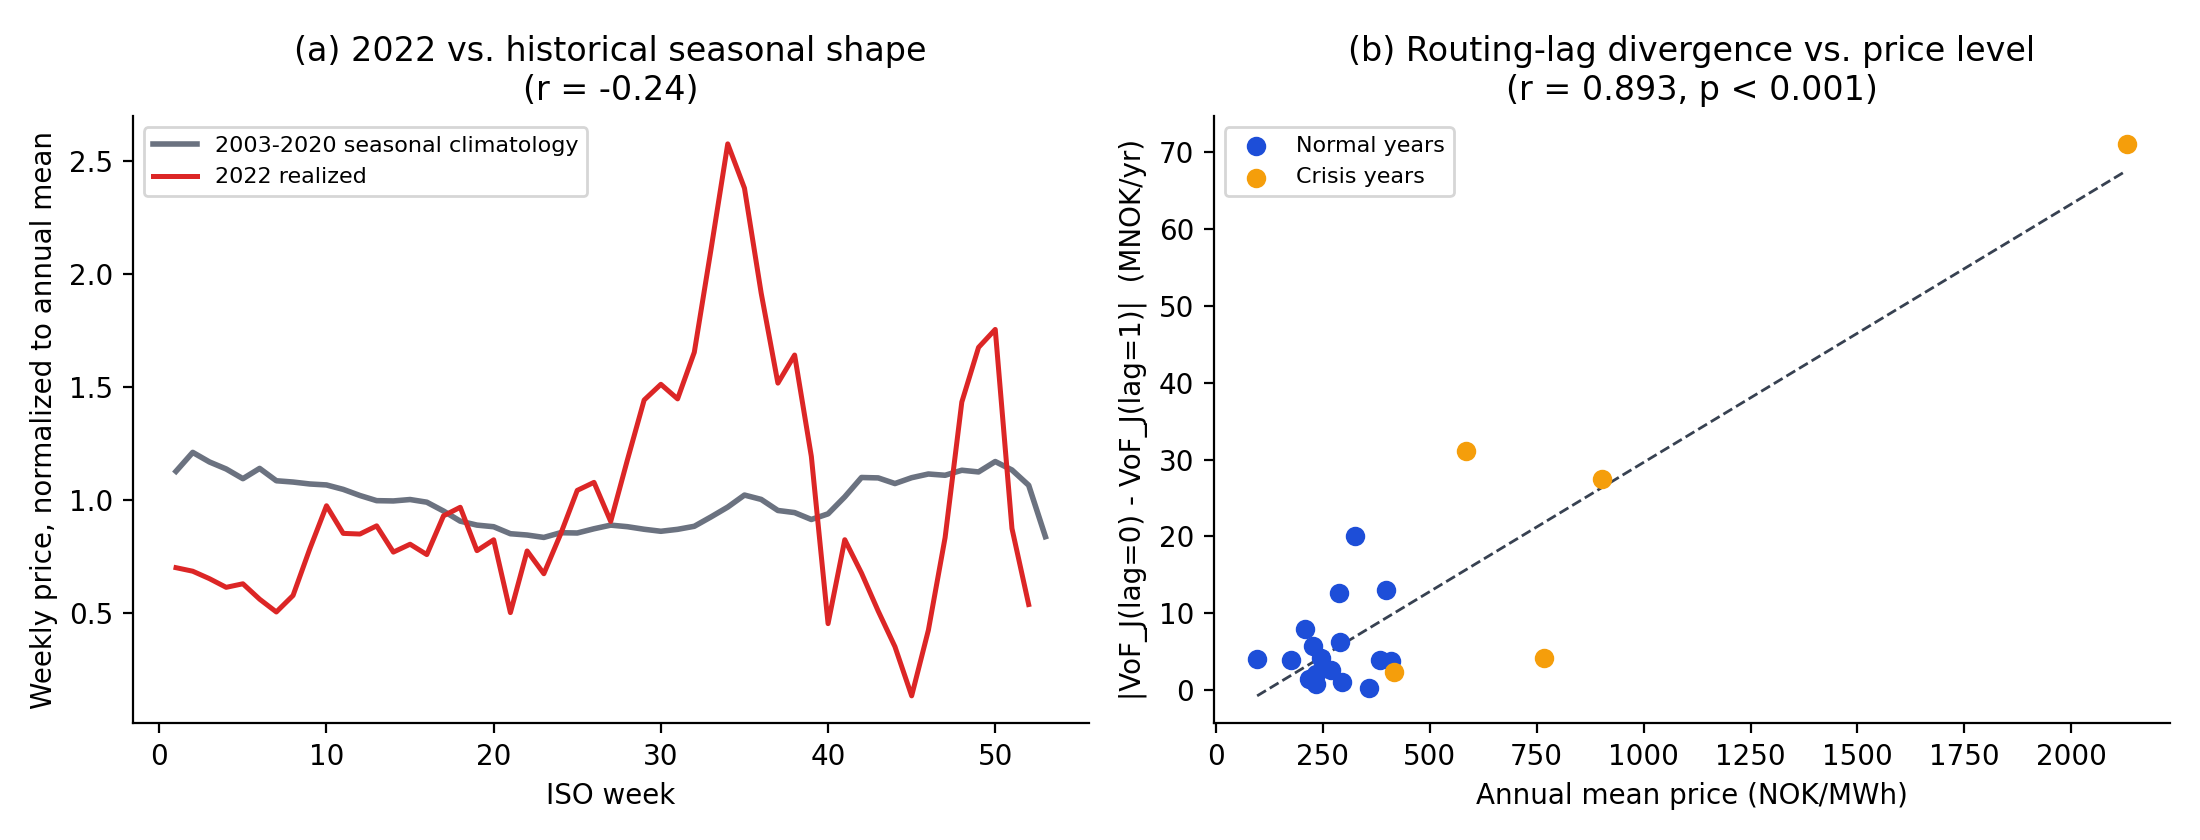
\includegraphics[width=\textwidth]{../results/figures/essay/fig2_regime_shift_mechanism.png}
\caption{(a) 2022 realized weekly price, normalized to its own annual mean, against the 2003-2020 seasonal climatology. (b) The absolute divergence between the lag-0 and lag-1 VoF$_J$ estimate, plotted against each year's annual mean price.}
\label{fig:regime-mechanism}
\end{figure}

The same qualitative breakdown, large and unstable estimates concentrated in the crisis years, also turns up independently in the earlier single-reservoir model. The two models are different enough in scale, head, and how storage is aggregated that their absolute numbers should not be compared directly, and a correction is worth making explicit here: an earlier pass at this analysis suggested the crisis-year VoF swings scaled almost exactly with the difference in reservoir size between the two models, and that does not survive a closer check. The storage ratio between the two models is about 7.8, the observed VoF ratio in crisis years is closer to 4. What does hold up, and what seems like the genuinely interesting part, is that the same kind of breakdown shows up at both levels of detail, which suggests this is a property of forecasting against a regime nobody planned for, not a quirk of one particular model's construction.

\section{Discussion}

Put together, these results say something a bit deflating but useful: a single multi-year average value-of-flexibility number can hide more than it reveals. The full 22-year average at Jorundland, $+0.99$ MNOK per year, sits close in sign to the normal years' average, but that is closer to luck than to insight, since the crisis years are not quietly near zero. They are wildly scattered, and happen to average out that way in this particular 22-year window. Anyone leaning on a number like this for an investment decision or a regulatory filing should ask, before trusting it, whether a handful of unusual years are doing all the work.

The concentration result has a more practical reading for anyone building or maintaining a model of a real cascade: do not bother looking for flexibility value at a run-of-river plant. It is not a matter of unlikely, it is structurally guaranteed to be exactly zero whenever local inflow clears turbine capacity, and that condition can be checked from historical flow records alone, with no optimization required. Whatever budget exists for computing this kind of quantity in a real system is better spent entirely on the nodes that actually hold water.

A few limitations are worth being upfront about. The closed-loop policy here is a rolling-horizon approximation, not full SDDP, so the flexibility values reported should be read as a floor, not a ceiling, on what a properly implemented recursive method would find. The routing lag between plants is a modeling assumption, same-week or one-week, rather than a measured hydraulic travel time, which was not available from public sources; it does not change the normal-year result, but its interaction with extreme prices, discussed above, should be read as a sensitivity rather than a settled fact. The Magasinstatistikk filling data used for initial storage is at NO2 zone resolution rather than specific to this watercourse, which adds some noise to each year's starting point that this analysis cannot remove.

The obvious next step, which this paper does not attempt, is to redo the closed-loop side with actual SDDP and see whether the normal-year premium grows once the policy can fully exploit recourse, and whether the crisis-year instability softens once the terminal value function is handled properly instead of approximated.

\section*{Bibliography}

The following are the real researchers, institutions, and methodological frameworks this work is positioned against, identified during earlier stages of this project. Specific titles, years, and venues below have not been independently re-verified against the original sources for this draft and should be checked before any external submission.

\begin{itemize}
\item Tomasgard, A., Crespo del Granado, P., and collaborators (NTNU/SINTEF). The EMPIRE model for multi-horizon capacity expansion planning under uncertainty.
\item Helseth, A., and Mo, B. SHOP: short-term and medium-term optimal hydropower scheduling, and the associated SDDP-based methodology used in Norwegian hydropower scheduling practice.
\item Fleten, S.E., and Kristoffersen, T.K. Stochastic programming for bidding strategies of a Nordic hydropower producer, \emph{European Journal of Operational Research}.
\item Birge, J.R., and Louveaux, F. \emph{Introduction to Stochastic Programming} (textbook reference for multistage stochastic programming and non-anticipativity).
\item Heitsch, H., and R\"omisch, W. Scenario reduction methods for stochastic programming, \emph{Computational Optimization and Applications} (methodological basis for the scenario tree reduction used in this project's forecasting pipeline).
\end{itemize}

\emph{Flag: every entry above needs a full bibliographic check (exact year, volume, page numbers, and confirmation the cited work says what it is being cited for) before this document could be submitted anywhere. None of the underlying empirical results in Sections 4 or 5 depend on these citations being correct; they are positioning context only.}

\end{document}
